\newpage
\subsubsection{UC7.2 - Visualizzazione Proprio Profilo Utente}
\label{UC7.2}

\begin{figure}[ht]
	\centering
	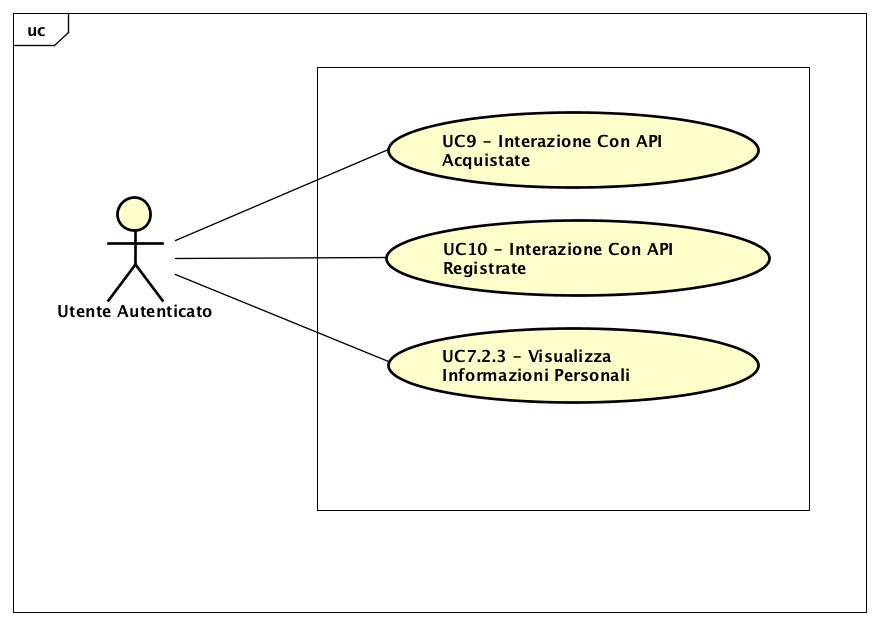
\includegraphics[scale=0.45]{UML/UC7_2.png}
	\caption{UC7.2 - Visualizzazione Proprio Profilo Utente}
\end{figure}
\FloatBarrier
\begin{longtable}{ l | p{11cm}}
	\hline
	\rowcolor{Gray}
	 \multicolumn{2}{c}{UC7.2 - Visualizzazione Proprio Profilo Utente} \\
	 \hline
	 \textbf{Attori} & Utente autenticato \\
	\textbf{Descrizione} & L’utente pu\'{o} visualizzare le proprie informazioni personali, interagire con le API da lui registrate e con le API acquistate  \\
	\textbf{Pre-Condizioni} & L’Utente \`{e} nel proprio profilo \\
	\textbf{Post-Condizioni} & L’Utente ha scelto l'interazione con il proprio profilo \\
	\textbf{Scenario Principale} & 
	\begin{enumerate*}[label=(\arabic*.),itemjoin={\newline}]
		\item L'utente pu\`{o} interagire con le API acquistate (UC9)
		\item L'utente pu\`{o} interagire con le API registrate (UC10)
		\item L'utente pu\`{o} visualizzare le Informazioni personali (UC7.2.3)
	\end{enumerate*}\\
\end{longtable}


